\section{Descrizione architettura }
	\subsection{Metodo e formalismo di specifica}
Le scelte architetturali per lo sviluppo di SWEDesigner sono state fortemente influenzate dallo stack tecnologico utilizzato. \\

Nell’esposizione dell’architettura dell'applicazione si procederà con un approccio \glossaryItem{top-down}, descrivendo l'architettura iniziando dal generale ed andando al particolare; si è partiti suddividendo il sistema in \glossaryItem{front-end} e \glossaryItem{back-end}, definendo l'interfaccia di comunicazione, scegliendo di seguire in ciascuno l'organizzazione suggeritaci dai \glossaryItem{framework}.

La descrizione dell’architettura di SWEDesigner è suddivisa in quattro sezioni:
\begin{itemize}
\item \S\ref{3.2}: illustra gli aspetti generali dell’architettura del software;
\item \S\ref{3.3}: descrive il protocollo che lega le due interfacce tra \glossaryItem{Client} e \glossaryItem{Server};
che descrive l’architettura del front end dell’applicazione;
\item \S\ref{3.4}: descrive l’architettura del \glossaryItem{back-end} dell’applicazione;
\item \S\ref{3.5}: descrive l’architettura del \glossaryItem{front-end} dell’applicazione.

\end{itemize}

Per descrivere in maniera formale l'architettura verranno impiegati lo standard \glossaryItem{UML} 2.0 per i diagrammi dei \glossaryItem{package} e delle classi e lo standard \glossaryItem{UML} 2.5 per i \glossaryItem{diagrammi di attività} e sequenza.

I diagrammi delle \glossaryItem{classi} che permettono di mostrare l'architettura generale del sistema vengono affiancati anche dai diagrammi di sequenza e attività, che permettono di definire le interazioni tra le componenti, senza preoccuparsi della loro classificazione.
In questo modo è possibile esprimere alcuni meccanismi tipici di un’applicazione
\glossaryItem{REST}-like, come il modo in cui agiscono i \glossaryItem{middleware}.

	\subsection{Architettura generale}
	\label{3.2}
	L'architettura del progetto si divide in una componente \glossaryItem{Client}, rappresentata da un'applicazione
\glossaryItem{front-end} accessibile da un browser, e in una componente Web\glossaryItem{Server}, nella quale risiede il \glossaryItem{back-end} che gestisce le richieste di generazione del \glossaryItem{codice}.\\
L'architettura generale di SWEDesigner si divide in 3 macrocomponenti:
\begin{itemize}
\item \textbf{\glossaryItem{Client}};
\item \textbf{\glossaryItem{Server} \glossaryItem{REST}};
\item \textbf{\glossaryItem{Database}}.
\end{itemize}

 \begin{figure}[h!]
\centering
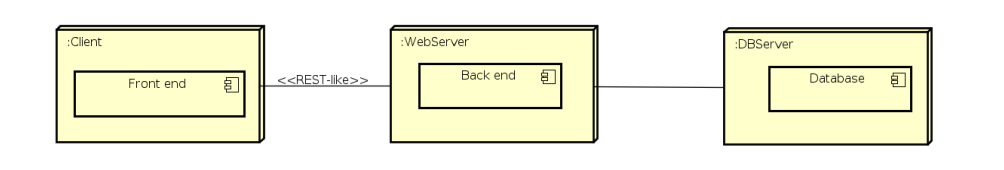
\includegraphics[scale=0.4]{Disegnetti/architetturaGenerale.png}
\caption{Diagramma di \glossaryItem{deployment} per l'architettura}
 \end{figure}

L'architettura proposta segue il \glossaryItem{Design Pattern} \emph{Three-tier}. Esso è diviso in 3 livelli:
\begin{itemize}
\item \textbf{Presentation tier}: rappresenta l'interfaccia verso l'utente ovvero lil \glossaryItem{front-end};
\item \textbf{Business logic}: è il livello che coordina l'applicazione ed effettua quindi le decisioni logiche e le valutazioni ovvero il \glossaryItem{back-end};
\item \textbf{Data tier}: è il livello dove le informazioni vengono salvate, ovvero il \glossaryItem{database}.
\end{itemize}


In particolare i ruoli di Model e Controller verranno implementati a livello di \glossaryItem{server}, mentre il ruolo di View viene affidato al \glossaryItem{front-end}. L'interfaccia tra le due componenti verrà gestita grazie ad un set di \glossaryItem{API} disposto dal \glossaryItem{server} \glossaryItem{REST}; il \glossaryItem{Database} serve per garantire la persistenza del programma generato: ogni \glossaryItem{utente} autenticato può salvare i propri progetti e mantenere i diagrammi creati.\\
Le tre macrocomponenti verranno descritte in dettaglio in seguito su questo documento.
	\subsection{Interfaccia REST-like}
	\label{3.3}
	Per l'interfaccia della componente \glossaryItem{back-end} si è scelto di utilizzare uno stile basato REST. All'interno di un’unica sessione utente, a partire dall’operazione di login fino a quella di logout, l'interfaccia con cui si accede agli elementi delle collection può considerarsi effettivamente REST.\\
I motivi che hanno spinto alla scelta di RESTsono:
\begin{itemize}
\item Semplicità di utilizzo;
\item Facile integrazione con i \glossaryItem{framework} esistenti;
\item Indipendenza dal linguaggio di programmazione utilizzato.
\end{itemize}
REST utilizza il concetto di risorsa, ovvero un aggregato di dati con un nome (URI) e una rappresentazione, su cui è possibile invocare le operazioni CRUD tramite la seguente corrispondenza:
	\subsection{Architettura del Server}
	\label{3.4}
	L'implementazione scelta per il backend dell'applicazione è un server che segue lo stile architetturale \glossaryItem{REST}; ciò implica che:
	\begin{itemize}
	\item l'applicazione renda disponibili le sue funzioni in veste di risorse web;
	\item ogni risorsa resa disponibile è indirizzabile univocamente utilizzando un indirizzo URL;
	\item l'interfaccia delle risorse deve essere uniforme e deve garantire un insieme ben definito di operazioni e una gestione priva di stato delle operazioni.
	\end{itemize}

Tale architettura permette l'indipendenza completa tra \glossaryItem{back-end} e \glossaryItem{front-end}, permettendo così espansioni su altre piattaforme senza dover modificare il \glossaryItem{back-end} dell'applicazione.
Il collegamento tra il \glossaryItem{front-end} e i modelli nel \glossaryItem{back-end} verrà implementato da uno stack di \glossaryItem{middleware}.
	\subsection{Architettura del Client}
	\label{3.5}
	Il \glossaryItem{front-end} di SWEDesigner è una \glossaryItem{Single Page Application}
	realizzata nel framework Angular4.0. L'architettura è MVVM (\emph{Model-View-View Model}),
	sono descritti due package principali Components e Services, i Components costituiscono
	la parte Viewmodel dell'architettura, contiene classi atte a rendere dinamica la pagina web;
	il package Services, che ripecchia la parte Model, offre metodi per l'interazione con il
	lato server e la libreria grafica. La parte View non viene descritta in quanto composta da
	 template html statici che sono strettamente legati	omonimi components.
